\documentclass[11pt]{article}

\usepackage[margin=1in]{geometry}
\usepackage{booktabs}
\usepackage{graphicx}
\usepackage{hyperref}
\usepackage{amsmath,amssymb}
\usepackage{xcolor}
\usepackage{multirow}
\usepackage{array}
\usepackage{setspace}
\usepackage[numbers,sort&compress]{natbib}
\usepackage{hyperref}

\hypersetup{colorlinks=true,linkcolor=black,citecolor=blue,urlcolor=blue}
\setstretch{1.05}

\title{Difficulty Sensitivity versus Ranking Stability in\\
Range-Constrained Combinatorial Search:\\
NutriOpt-Bench for Evolutionary Computation}
\author{
NutriOpt-Bench Project\\
\textit{IEEE TEVC reconstruction --- evidence-driven draft after complete E1--E4 PRIMARY.}
}
\date{\today}

\begin{document}
\maketitle

\begin{abstract}
Constrained combinatorial search often couples large binary decision spaces with coupled interval constraints and potentially sparse feasible regions.
Range-constrained food assembly (RCFA)---selecting a subset of foods whose nutrient totals fall inside prescribed intervals---is a transparent real-world instance of this regime, yet published diet-planning studies are incommensurate in representation, constraint geometry, and evaluation protocol.
We present NutriOpt-Bench, a fair-budget evolutionary benchmark that independently varies food-space scale, interval constraint tightness, and nutrient dimensionality under identical evaluation budgets ($100{,}000$ evaluations; population $500$; $10$ seeds).
Across completed PRIMARY campaigns, interval tightness produced the largest change in feasibility: mean feasible-hit rate (FHR) rose from $0.172$ under tight intervals to $0.962$ under relaxed intervals.
In contrast, NHANES scaling from $5$K to approximately $210$K candidates maintained mean FHR in the $0.76$--$0.82$ range under the same budget, indicating that nominal decision-space scale alone is not a sufficient predictor of feasibility difficulty here.
Constraint dimensionality remained near ceiling through nine nutrients and became substantially heterogeneous at sixteen nutrients.
Despite these changes in absolute difficulty, cross-regime rankings among shared algorithms were highly concordant (Kendall $\tau=0.909$--$0.982$).
Feasibility-oriented/memetic methods (MA, ACMO-Diet, BMOEA) together with NSGA-II formed a relatively stable leading group, while random search remained consistently weak.
The central implication for evolutionary computation is a separation between \emph{difficulty sensitivity} and \emph{ranking sensitivity}: harder regimes need not imply wholesale reordering of algorithmic effectiveness.
\end{abstract}

\section{Introduction}
Constrained combinatorial optimization frequently combines binary decisions, coupled constraints, and sparse feasible sets.
Diet planning provides a concrete instantiation: assemble a meal or daily selection so that aggregate nutrients lie in dietary intervals, optionally with structural coverage (e.g., meals).
Classical linear programs~\citep{stigler1945,smith1959} and evolutionary menu planners~\citep{gaal2005,seljak2006} address related tasks, while multiobjective evolutionary algorithms (MOEAs)~\citep{deb2002,zhang2007,zitzler2001,cheng2016,li2019ctaea} supply the broader algorithmic repertoire.
However, existing comparisons rarely share instances, budgets, or metrics, so ``algorithm $A$ beats $B$'' claims do not transfer.

A deeper issue is conceptual.
When a problem regime becomes harder, two distinct phenomena may occur:
(i)~absolute performance deteriorates for many methods (\emph{difficulty sensitivity});
(ii)~the relative ordering of methods changes (\emph{ranking sensitivity}).
These need not coincide.
NutriOpt-Bench is designed to ask:

\begin{quote}
\emph{How do changes in problem-regime structure affect the absolute difficulty of evolutionary search, and to what extent do they alter the relative effectiveness of different evolutionary mechanisms?}
\end{quote}

\subsection{Research questions}
\begin{itemize}
\item \textbf{RQ1:} How can optimization-based diet planning be characterized by evolutionary-search-relevant structure?
\item \textbf{RQ2:} How does food-space scale affect feasibility discovery under a fixed evaluation budget?
\item \textbf{RQ3:} How strongly does interval constraint tightness alter feasible-solution discovery?
\item \textbf{RQ4:} How does increasing constraint dimensionality affect search?
\item \textbf{RQ5:} Are relative algorithm rankings stable across regimes?
\item \textbf{RQ6:} Which algorithmic families perform consistently well in difficult feasibility regimes?
\end{itemize}

\subsection{Contributions}
\begin{enumerate}
\item A structured taxonomy of optimization-based diet planning along representation, target geometry, structure, paradigm, and evaluation.
\item A frozen RCFA formulation and reproducible NutriOpt-Bench separating scale, interval tightness, and dimensionality under matched budgets.
\item PRIMARY evidence that interval tightness is the strongest tested difficulty axis; NHANES scale does not collapse FHR under $100$k evaluations; dimensionality becomes heterogeneous mainly at $16$ nutrients.
\item Cross-regime analysis showing high Kendall concordance of rankings despite large absolute FHR shifts---separating difficulty sensitivity from ranking sensitivity.
\end{enumerate}

\section{Structured Literature Analysis}
We follow a documented search protocol and seed coding matrix (\texttt{literature/}).
Landmarks include classical LP diets~\citep{stigler1945,smith1959}, evolutionary menu planning~\citep{gaal2005,seljak2006}, and methodological MOEAs~\citep{deb2002,zhang2007,zitzler2001,cheng2016,li2019ctaea}.
This is a \emph{structured literature analysis}, not a completed PRISMA systematic review: live database screening counts remain incomplete and are not claimed as finished.

\section{Taxonomy of Optimization-Based Diet Planning}
We organize prior work on five orthogonal axes (details in \texttt{literature/taxonomy.md}):
(1)~decision representation;
(2)~target geometry (point, one-sided, interval);
(3)~structural constraints;
(4)~optimization paradigm;
(5)~evaluation criteria.
RCFA occupies binary subset selection with interval boxes, optional meal coverage, and feasibility-first metrics.
These axes motivate NutriOpt-Bench factors: representation $\rightarrow$ binary foods; geometry $\rightarrow$ interval tightness; catalog size $\rightarrow$ scale; simultaneous nutrients $\rightarrow$ dimensionality.

\section{Range-Constrained Food Assembly}
\subsection{Core model}
Select $x\in\{0,1\}^N$ with nutrient matrix $A\in\mathbb{R}^{N\times m}$:
\begin{align}
K_{\min}\le \|x\|_0\le K_{\max},&\qquad
L_j\le \sum_i A_{ij}x_i\le U_j\quad(j\in J),\\
\sum_{i\in M_m}x_i\ge 1&\quad\text{(meals, when enabled)}.
\end{align}
Hard feasibility ignores soft diversity penalties.
Native solvers optimize a scalar penalty fitness; pymoo paths use a shared bi-objective decode.
Both realize the same binary selection semantics (\texttt{docs/RCFA\_FORMULATION.md}).

\subsection{What RCFA is not}
Continuous portion LPs, recommender-only systems, and clinical outcome evaluation are out of scope.
NutriOpt-Bench measures \textbf{optimization behavior}, not dietary adequacy.

\section{NutriOpt-Bench}
\subsection{Data and targets}
NHANES food instances ($\sim$210k rows, $16$ nutrients, meal tags) form the primary combinatorial regime.
Recipe catalogs ($\sim$1.5--1.8k foods, $4$ nutrients, no meals) are easy-regime calibrations and must be analyzed separately.
Representative targets (cluster-12) show lower mean nearest-neighbor distance than random-12 in a standardized feature proxy ($3.77$ vs.\ $4.54$; descriptive, not a statistical representativeness claim).

\subsection{Axes}
\textbf{E2} interval-width factors $\{0.5,1.0,1.5\}$ (interval-induced feasibility regimes; sanitized one-sided bounds).
\textbf{E1} food-space scale (recipe + NHANES samples/full).
\textbf{E3} nutrient dimensions $\{6,9,12,16\}$ via canonical prefix projection.
\textbf{E4} cross-regime meta-analysis (no new solver runs).

\subsection{Fairness}
PRIMARY: population $500$, $\texttt{max\_evaluations}=100{,}000$, $10$ seeds, early-stop disabled, hashed seeds.
Residual asymmetries: MA median $\approx 100.8$k and Greedy $\approx 100.2$k evaluations (inner scoring); RandomRepair uses full $100$k after correction.
We report matched budgets with documented residuals (\texttt{docs/FAIRNESS\_AUDIT.md}).

\subsection{Algorithms}
MA, ACMO-Diet, BMOEA, NSGA-II~\citep{deb2002}, SPEA2~\citep{zitzler2001}, RVEA~\citep{cheng2016}, C-TAEA~\citep{li2019ctaea}, Random, Greedy, RandomRepair (E3 omits Greedy/Repair).
MILP/CBC on reduced candidate pools provides feasibility calibration, not large-scale competition.

\section{Experimental Design}
Primary metric: feasible-hit rate (FHR).
Secondary: evaluations to first feasible (FFG\_evals), BestFit, runtime, recorded \texttt{n\_evals}.
Within each regime, Friedman tests on target-aggregated FHR assess ranking differences.
Across regimes, mean Friedman ranks and Kendall $\tau$ assess concordance.
Recipe and NHANES results are never pooled for ranking claims.

\section{Results}

\subsection{Overall feasibility landscape}
Figure~\ref{fig:concept} summarizes the empirical distinction between absolute difficulty and ranking stability.
The hardest PRIMARY cell is E2 with $f=0.5$ (mean FHR $0.172$); the easiest NHANES-like cells approach ceiling FHR under relaxed intervals or low dimension.

\begin{figure}[t]
\centering
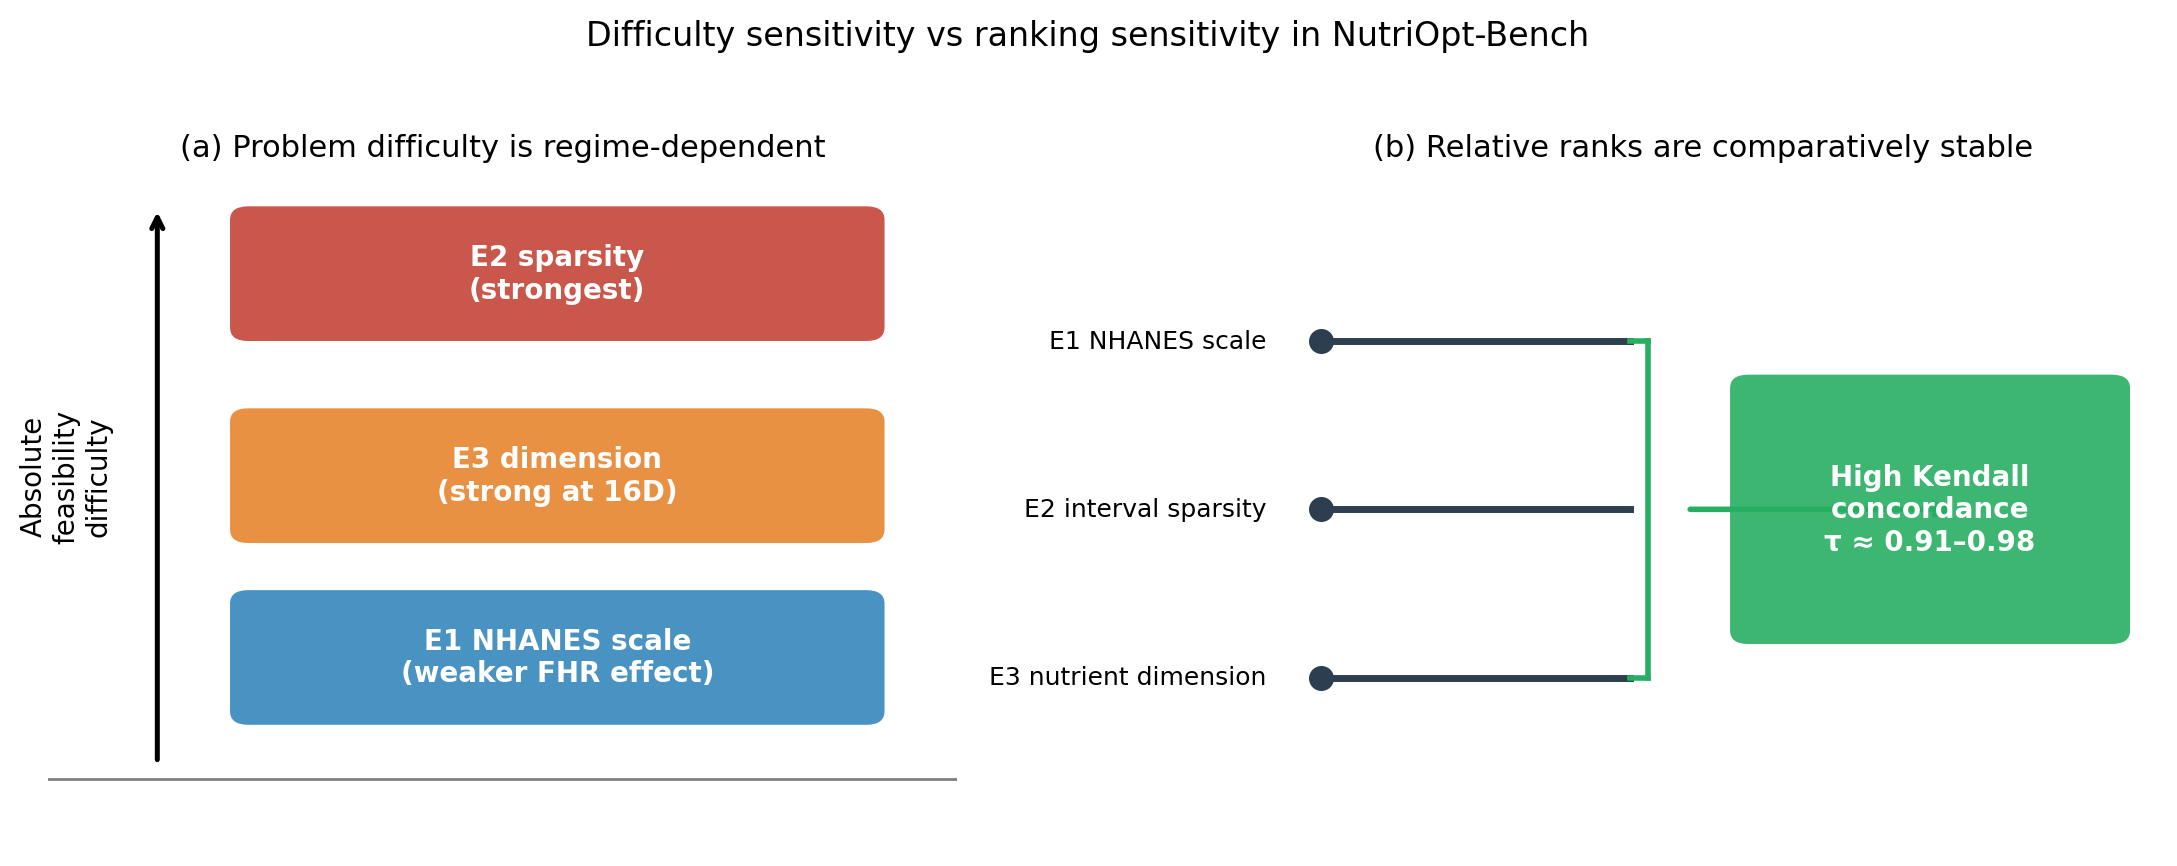
\includegraphics[width=\textwidth]{../results/figures/fig_tevc_difficulty_vs_ranking.png}
\caption{Conceptual summary of NutriOpt-Bench PRIMARY findings:
(a)~absolute feasibility difficulty is strongly regime-dependent;
(b)~relative algorithm ranks remain highly concordant (Kendall $\tau\approx 0.91$--$0.98$).}
\label{fig:concept}
\end{figure}

\subsection{Constraint tightness as the primary difficulty axis (E2)}
On NHANES-10K, mean FHR increased from $0.172$ ($f=0.5$) to $0.761$ ($f=1.0$) to $0.962$ ($f=1.5$) (Fig.~\ref{fig:e2}).
Friedman tests reject equal algorithm performance at all three factors ($p=1.8\times10^{-3}$, $1.1\times10^{-9}$, $6.6\times10^{-3}$).
At tight intervals, even $100$k evaluations yield low hit rates; MA ($0.275$) and RandomRepair ($0.242$) lead, while Random is near zero ($0.017$).
At $f=1.5$, several structured methods reach FHR $=1.0$.
We interpret $f$ as inducing distinct \emph{interval-induced feasibility regimes}, not as a directly measured geometric density unless density probes are cited separately.

\begin{figure}[t]
\centering
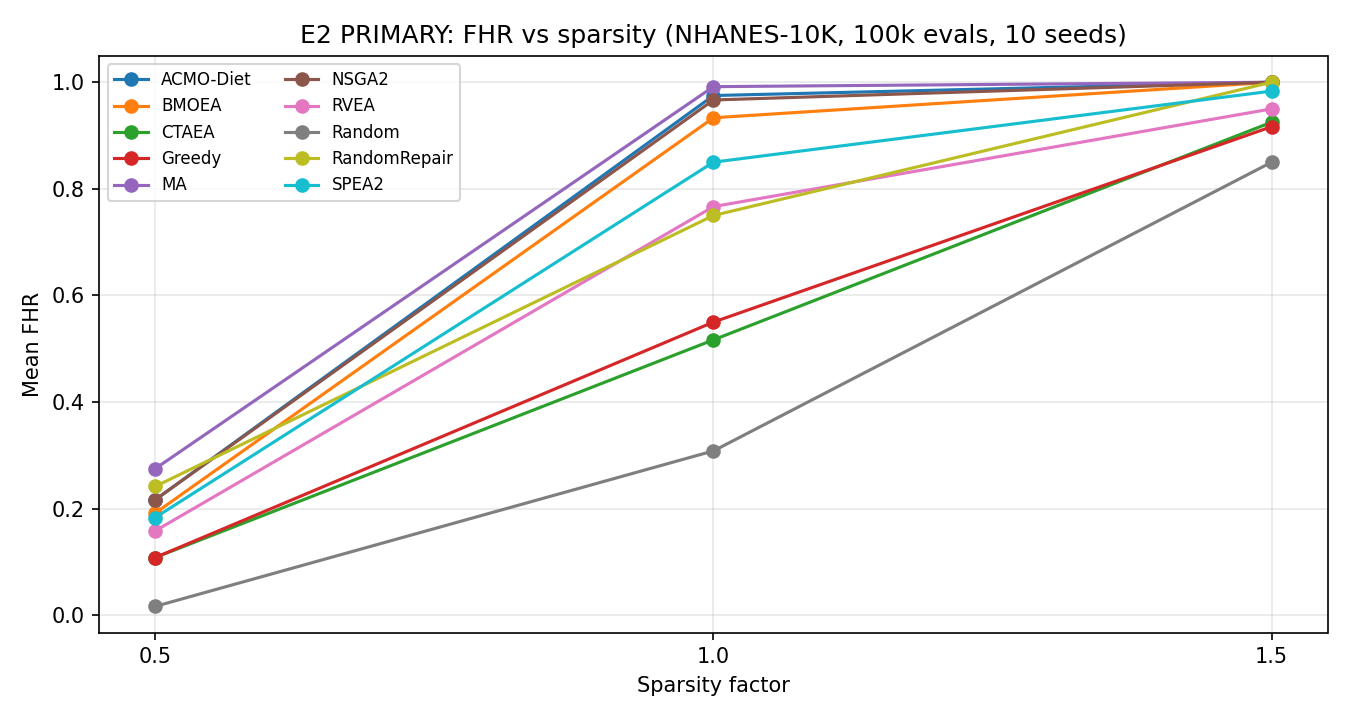
\includegraphics[width=0.85\textwidth]{../results/figures/fig_e2_full_fhr_sparsity.png}
\caption{E2 PRIMARY: mean FHR versus interval-width factor (NHANES-10K; $100$k evaluations; $10$ seeds).}
\label{fig:e2}
\end{figure}

\subsection{Search-space scaling (E1)}
Recipe catalogs yield FHR $=1.000$ for every algorithm---a ceiling regime that must not support superiority claims.
On NHANES, mean FHR across algorithms remains approximately $0.76$--$0.82$ from $5$K to full ($\approx 210$K) under the fixed $100$k budget (Fig.~\ref{fig:e1}).
We do \textbf{not} claim monotonic FHR decrease with $N$.
Within the tested range, increasing catalog size did not produce an FHR collapse; algorithm gaps remain large and Friedman-significant at every scale ($p\sim 10^{-9}$--$10^{-10}$).
Scale still affects wall-clock cost and per-evaluation work; it is simply a weaker predictor of FHR than interval tightness here.

\begin{figure}[t]
\centering
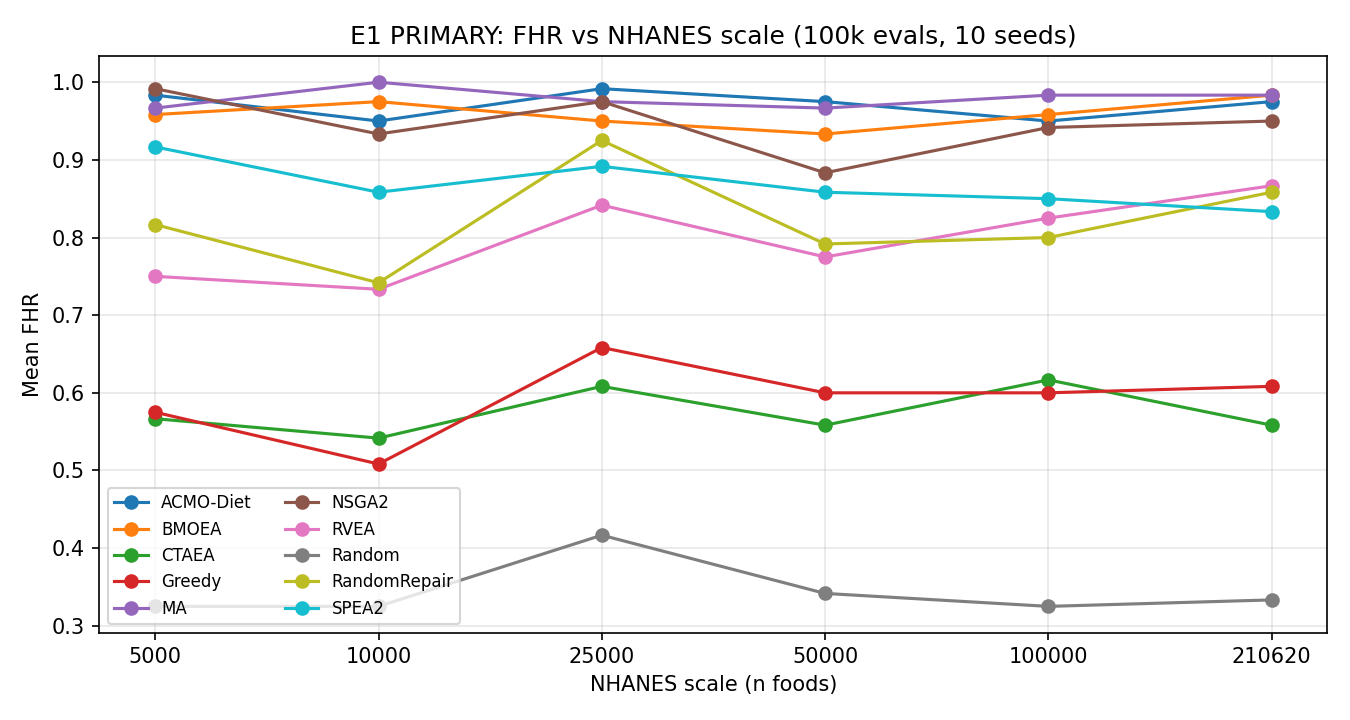
\includegraphics[width=0.85\textwidth]{../results/figures/fig_e1_full_fhr_scale.png}
\caption{E1 PRIMARY: mean FHR versus NHANES food-space scale ($100$k evaluations; $10$ seeds).}
\label{fig:e1}
\end{figure}

\subsection{Constraint dimensionality (E3)}
Mean FHR is near ceiling at $6$ and $9$ nutrients ($0.992$, $0.983$), dips modestly at $12$ ($0.946$), and becomes substantially heterogeneous at $16$ ($0.795$) (Fig.~\ref{fig:e3}).
Friedman is non-significant at dim~$6$ (ceiling) and significant at $9$/$12$/$16$ (strongest at $16$, $p\approx 10^{-8}$).
At dim~$16$, MA/ACMO/BMOEA/NSGA2 remain strong; Random ($0.300$), C-TAEA ($0.592$), and RVEA ($0.733$) degrade.
We describe a \emph{threshold-like practical effect} in the tested setting, not a mathematically established phase transition.
\textbf{Construction note:} nutrients absent from a representative target are completed with $[0,\mathrm{empirical\_cap}]$ before prefix projection; this design choice is necessary for uniform dimensionality but is not a purely natural dietary formulation.

\begin{figure}[t]
\centering
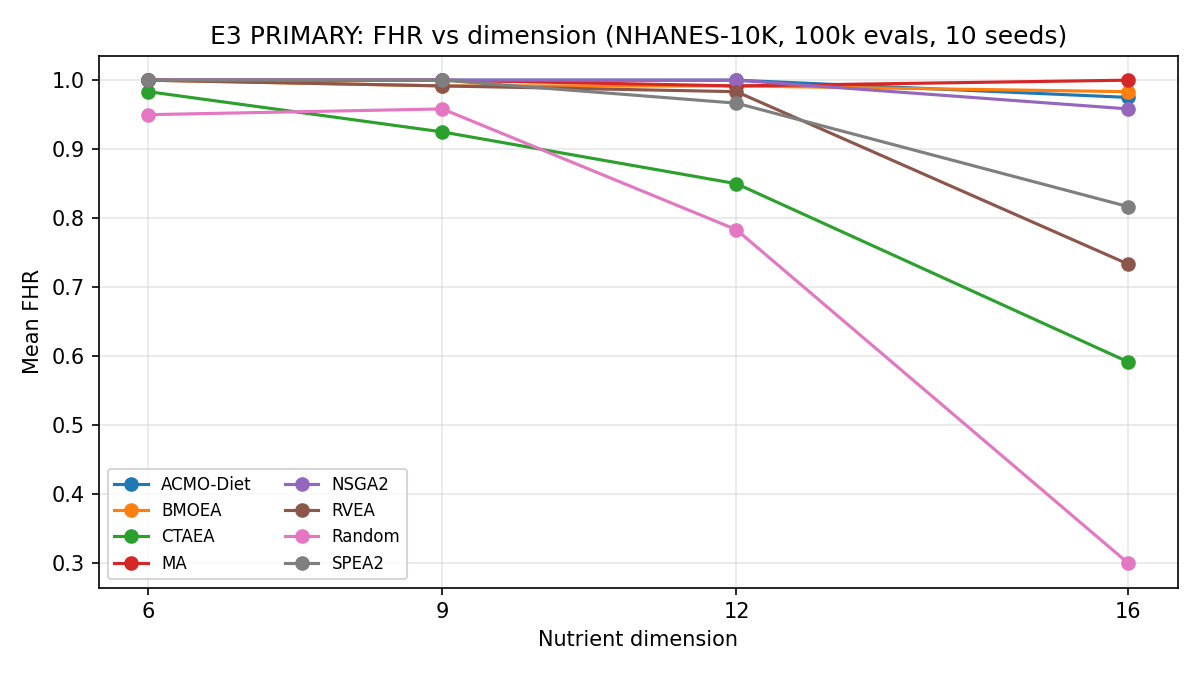
\includegraphics[width=0.85\textwidth]{../results/figures/fig_e3_full_fhr_dim.png}
\caption{E3 PRIMARY: mean FHR versus nutrient dimension (NHANES-10K; $100$k evaluations; $10$ seeds).}
\label{fig:e3}
\end{figure}

\subsection{Cross-regime ranking stability (E4)}
E4 aggregates E1 NHANES, E2, and E3 without new runs.
Cross-regime mean Friedman ranks (Table~\ref{tab:ranks}; Fig.~\ref{fig:e4ranks}) place MA ($3.94$), ACMO-Diet ($4.07$), NSGA2 ($4.14$), and BMOEA ($4.34$) as a leading group; Random is last ($7.13$).
Among eight shared algorithms, Kendall concordance is high and significant:
E1--E2 $\tau=0.982$ ($p=7.6\times10^{-4}$),
E1--E3 $\tau=0.929$ ($p=4.0\times10^{-4}$),
E2--E3 $\tau=0.909$ ($p=1.8\times10^{-3}$).
Thus absolute difficulty changes substantially, while relative ordering remains comparatively robust.
We do \textbf{not} claim wholesale rank reversal across regimes.

\begin{table}[t]
\centering
\caption{Cross-regime mean Friedman ranks (1 $=$ best). Overall averages non-missing cells.}
\label{tab:ranks}
\begin{tabular}{lcccc}
\toprule
Algorithm & E1 NHANES & E2 sparsity & E3 dim & Overall \\
\midrule
MA & 3.69 & 4.24 & 3.89 & \textbf{3.94} \\
ACMO-Diet & 3.81 & 4.50 & 3.90 & 4.07 \\
NSGA2 & 3.96 & 4.50 & 3.96 & 4.14 \\
BMOEA & 4.24 & 4.74 & 4.04 & 4.34 \\
SPEA2 & 4.78 & 5.22 & 4.23 & 4.74 \\
RandomRepair & 4.90 & 5.21 & --- & 5.06 \\
RVEA & 5.94 & 6.08 & 4.59 & 5.54 \\
CTAEA & 7.88 & 6.82 & 5.79 & 6.83 \\
Greedy & 7.28 & 6.42 & --- & 6.85 \\
Random & 8.52 & 7.28 & 5.60 & 7.13 \\
\bottomrule
\end{tabular}
\end{table}

\begin{figure}[t]
\centering
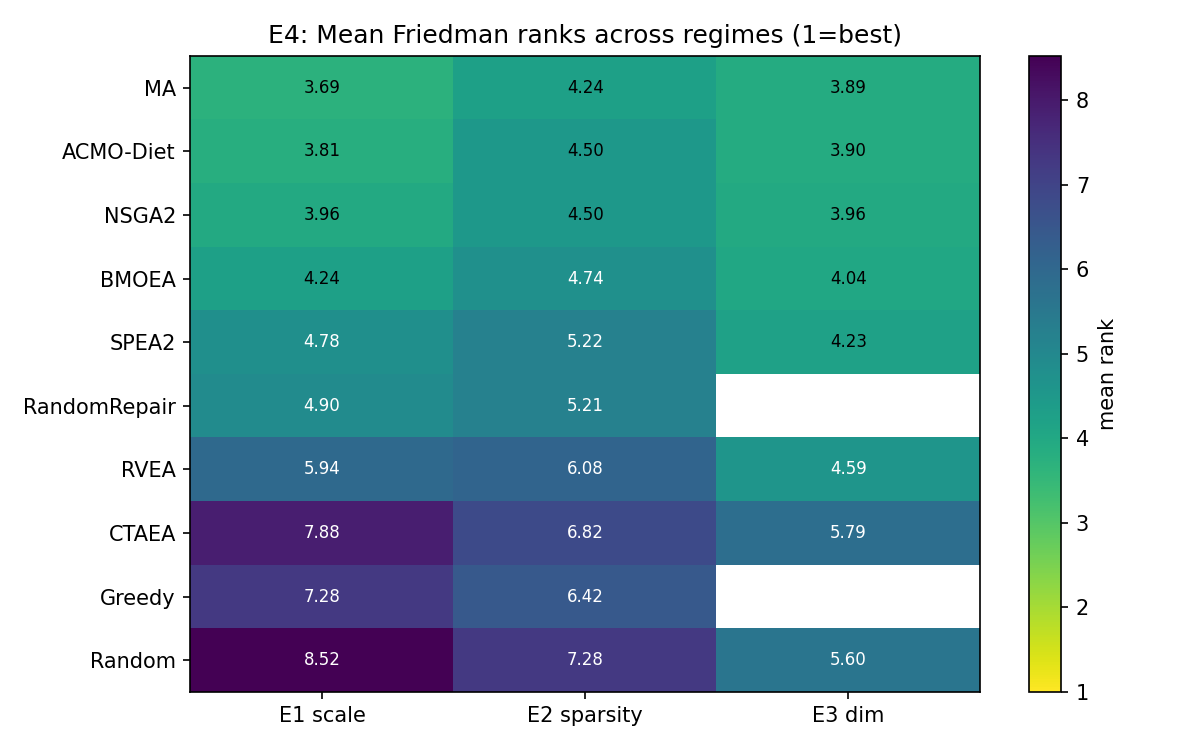
\includegraphics[width=0.72\textwidth]{../results/figures/fig_e4_cross_regime_ranks.png}
\caption{E4: mean Friedman ranks across E1--E3 regimes (1 $=$ best).}
\label{fig:e4ranks}
\end{figure}

\subsection{Search dynamics and mechanistic interpretation}
A limited dynamics probe (BMOEA vs.\ Random on one NHANES subsample) exists under \texttt{results/raw/trajectories/}; PRIMARY campaigns do not log full generation trajectories for all runs.
We therefore do not claim comprehensive dynamics conclusions.
Empirically, feasibility-oriented/memetic methods and NSGA-II form a stable leading group.
This is \emph{consistent with} the hypothesis that local improvement and feasibility pressure help in interval-constrained subset search, but without ablations we treat mechanism stories as interpretive rather than causal.

\subsection{Exact feasibility calibration}
On NHANES-500 with candidate limit $300$, CBC returned Optimal for all $12$ representatives; four remained nutritionally infeasible (\texttt{rep\_000}, \texttt{005}, \texttt{008}, \texttt{011}).
Zero FHR can therefore reflect empty feasible sets rather than evolutionary failure.
MILP is used only as small-instance calibration.

\subsection{Target robustness}
Cluster-12 coverage is a descriptive proxy favoring broader local coverage than random-12 under the adopted features; it is not claimed as statistical representativeness of all dietary targets.

\section{Discussion}
\subsection{What determines difficulty?}
In the tested FHR regime, interval-induced tightness dominates nominal food-space scale.
High constraint dimensionality matters mainly at $16$ nutrients.
Benchmark cells with near-universal FHR $\approx 1$ (recipes; low-dim E3) provide little discrimination.

\subsection{Does harder search change rankings?}
Not dramatically for the shared algorithm set: Kendall $\tau$ remains high.
Difficulty sensitivity and ranking sensitivity are empirically separable here.

\subsection{Evolutionary mechanisms}
Leading performance of MA/ACMO/BMOEA/NSGA2 across hard cells is evidence-consistent with feasibility-oriented search being advantageous, not a proof of theoretical superiority.
Random's stable gap indicates exploitable combinatorial structure relative to unstructured sampling.

\subsection{Implications for EC and beyond}
Benchmarks should vary both absolute difficulty and ranking sensitivity.
Structurally related domains (subset selection, resource allocation, constrained configuration) share ingredients of RCFA but were not evaluated here.

\section{Practical Algorithm Selection}
Empirical, benchmark-derived guidance only:
\begin{itemize}
\item Difficult feasibility regimes ($f=0.5$; dim~$16$): prefer MA / ACMO-Diet / BMOEA / NSGA-II.
\item Easy ceiling regimes (recipes; low dim): algorithm choice is less consequential for FHR.
\item Random is not recommended when structured search is required; Greedy is not competitive with the leading group on NHANES PRIMARY.
\item RandomRepair is competitive in some settings under equal budgets.
\end{itemize}
No universal champion is declared.

\section{Limitations}
Incomplete PRISMA screening; E3 empirical-cap padding; CTAEA/pymoo residual asymmetries; limited PRIMARY trajectory logging; soft-only diversity; no preference/cost/allergy axes; exploratory E4 curve-collapse/ADI/$N^*$ fits are unstable and relegated to supplement---no scaling phase boundary is claimed.

\section{Conclusion}
RCFA provides a controlled large-scale range-constrained combinatorial regime for evolutionary computation.
Within NutriOpt-Bench PRIMARY, interval tightness most strongly modulates absolute FHR; NHANES scale alone does not collapse FHR under $100$k evaluations; dimensionality becomes heterogeneous mainly at $16$ nutrients.
MA, ACMO-Diet, NSGA-II, and BMOEA form a relatively stable leading group, and cross-regime Kendall concordance is high ($\tau=0.909$--$0.982$).
Thus, under the tested budgets and algorithms, changes in problem difficulty do not necessarily imply changes in relative algorithm ranking---a separation between difficulty sensitivity and ranking sensitivity.

\section*{Data and Code}
Repository \texttt{nutri-range-opt-survey}.
PRIMARY CSVs under \texttt{results/raw/}; reports under \texttt{results/statistics/}; freezes in \texttt{docs/}.

\begin{thebibliography}{99}
\bibitem[Cheng et~al.(2016)]{cheng2016}
R.~Cheng, Y.~Jin, M.~Olhofer, and B.~Sendhoff.
\newblock A reference vector guided evolutionary algorithm for many-objective optimization.
\newblock {\em IEEE Transactions on Evolutionary Computation}, 20(5):773--791, 2016.

\bibitem[Deb et~al.(2002)]{deb2002}
K.~Deb, A.~Pratap, S.~Agarwal, and T.~Meyarivan.
\newblock A fast and elitist multiobjective genetic algorithm: NSGA-II.
\newblock {\em IEEE Transactions on Evolutionary Computation}, 6(2):182--197, 2002.

\bibitem[Ga\'{a}l et~al.(2005)]{gaal2005}
B.~Ga\'{a}l, I.~Vass\'{a}nyi, and G.~Kozmann.
\newblock A novel artificial intelligence method for weekly dietary menu planning.
\newblock {\em Methods of Information in Medicine}, 44(5):655--664, 2005.

\bibitem[Li et~al.(2019)]{li2019ctaea}
K.~Li, R.~Chen, G.~Fu, and X.~Yao.
\newblock Two-archive evolutionary algorithm for constrained multiobjective optimization.
\newblock {\em IEEE Transactions on Evolutionary Computation}, 23(2):303--315, 2019.

\bibitem[Seljak(2006)]{seljak2006}
B.~K.~Seljak.
\newblock Computer-based dietary menu planning.
\newblock {\em Journal of Food Composition and Analysis}, 19(6--7):687--695, 2006.

\bibitem[Smith(1959)]{smith1959}
V.~E.~Smith.
\newblock Linear programming models for the determination of palatable human diets.
\newblock {\em Journal of Farm Economics}, 41(2):272--283, 1959.

\bibitem[Stigler(1945)]{stigler1945}
G.~J.~Stigler.
\newblock The cost of subsistence.
\newblock {\em Journal of Farm Economics}, 27(2):303--314, 1945.

\bibitem[Zhang and Li(2007)]{zhang2007}
Q.~Zhang and H.~Li.
\newblock MOEA/D: A multiobjective evolutionary algorithm based on decomposition.
\newblock {\em IEEE Transactions on Evolutionary Computation}, 11(6):712--731, 2007.

\bibitem[Zitzler et~al.(2001)]{zitzler2001}
E.~Zitzler, M.~Laumanns, and L.~Thiele.
\newblock SPEA2: Improving the strength Pareto evolutionary algorithm.
\newblock TIK-Report 103, ETH Zurich, 2001.
\end{thebibliography}

\appendix
\section{Supplementary pointers}
Extended tables, exploratory E4 diagnostics (curve-collapse, ADI, unstable $N^*$ fits), parameters, and reproducibility commands: \texttt{manuscript/supplementary.tex}, \texttt{docs/}, \texttt{results/}.

\end{document}
